\documentclass{article}
\usepackage[a4paper,top=2cm,bottom=2cm,left=2cm,right=2cm]{geometry}
\usepackage[english]{babel}
\usepackage[T1]{fontenc}
\usepackage[utf8]{inputenc}
\usepackage{fancyhdr}
\usepackage{float}
\usepackage{graphicx}
\usepackage{wrapfig}
\usepackage{siunitx} %per scrivere il simbolo °
\usepackage{verbatim} %per i commenti1
\usepackage{subfig}
\usepackage{amsmath}
\usepackage{algorithm}
\usepackage{algpseudocode}
\setcounter{secnumdepth}{3}
\setcounter{tocdepth}{6}
\usepackage{multirow}
\newcommand{\minitab}[2][l]{\begin{tabular}#1 #2\end{tabular}}
\usepackage{rotating}
\usepackage{xfrac}
\usepackage{cite}

\DeclareMathOperator*{\argmax}{arg\,max}
\DeclareMathOperator*{\argmin}{arg\,min}

%\usepackage{booktabs,array}
%\usepackage{tikz}

%\usepackage{tabularx}

%\usepackage{chngcntr}
%\counterwithin{table}{section}

%------------------------------ colors
\usepackage[usenames,dvipsnames,table]{xcolor} % use colors on table and more
\definecolor{333}{RGB}{51, 51, 51} % define custom color
\definecolor{background}{RGB}{248, 248, 255}
\definecolor{comment}{RGB}{17,167,5}
\definecolor{keyword}{RGB}{195,47,8}
\definecolor{string}{RGB}{142,195,0}
\definecolor{number}{RGB}{90,84,84}
\definecolor{identifier}{RGB}{0,90,201}

%------------------------------ source code
\usepackage{listings}

\lstset{
  basicstyle=\footnotesize\sffamily,
  commentstyle=\itshape\color{gray},
  captionpos=b,
  frame=shadowbox,
  language=HTML,
  rulesepcolor=\color{333},
  tabsize=2
}

\lstdefinestyle{code}{
  backgroundcolor=\color{background},
  basicstyle=\footnotesize\sffamily,
  commentstyle=\color{comment},
  frame=L,
  identifierstyle=\color{identifier},
  keywordstyle=\color{keyword},
  numbers=left,
  numbersep=10pt,
  numberstyle=\tiny\color{number},
  stringstyle=\color{string},
  showstringspaces=false,  
  stepnumber=1,
  tabsize=2
}

\title{\textbf{Report about Lab5}} % Title
\author{Raffaele \textsc{Di Nardo Di Maio} 1204879} % Author name
\date{\today}

\begin{document}
\begin{minipage}{.20\textwidth}
  
\includegraphics[height=3cm]{../Icon4}
\end{minipage}\begin{minipage}{.20\textwidth}
  \begin{table}[H]
  \begin{tabular}{l}
  \scshape{\Large{Computer Engineering Master Degree}} \\
  \hline \\
  \scshape{\Large{Computer Vision}} \\
  \end{tabular}
  \end{table}
\end{minipage}
{\let\newpage\relax\maketitle}

\section{Goal of the experience}
The goal of this lab experience is to create a panoramic view by overlapping a set of images looking at their relative positions. To obtain them, I evaluate the translations between consecutive images. Hence I consider only the possibility of having a translation to the right of an image in the sequence w.r.t the previous one.  
\section{Code Organization}
The code of this lab is organized in 5 files (for which I provide also the documentation through doxygen):
\begin{itemize}
\item{\textbf{Lab5.cpp} and its header file \textbf{Lab5.h}.\\
They are associated to \texttt{main()} where two threads create instances of \texttt{PanoramicImage()} and call their function \texttt{panoramic\_view()} to create panoramic views using SIFT or ORB.}
\item{\textbf{PanoramicImage.cpp} and its header file \textbf{PanoramicImage.h}.\\
These are used to create the class \texttt{PanoramicImage} and other exception classes. Its main function is called \texttt{panoramic\_view()} and manages the main flow of the program, that is organized in four main phases:
\begin{enumerate}
\item{Projection of images on a cylindrical surface;}
\item{Computation of keypoints and descriptors for all images;}
\item{Computation of matches and inliers;}
\item{Computation of translations of an image w.r.t. the previous one.}
\end{enumerate}
\item{\textbf{PanoramicUtils.h}.\\
This is the file provided by professors to compute the cylindrical projection.}
}
\end{itemize}
\section{Command line parameters}
The program needs to have, as command line arguments, the path of the folder that contains the input images and the FOV of the camera.
\section{User interaction}
At runtime the user needs to insert the value of FOV, if a value less than 1 is provided on command line. Then the user needs to insert separately the ratios for the definition of the inliers for SIFT and ORB.
\section{Experimental results}
The program uses threads and computes simultaneously ORB and SIFT detections on BW images, after their cylindrical projection. The results with SIFT are better than ORB, but the computational load is heavier.\\
Each projected image is equalized to improve the final result, that is equalized too. The final panoramic image for each detection method, is made through mean translations of the previously computed projected images.\\
Negative translations on x axis are considered as an error hence I transform them into translations of norm equal to the width of the previous image.\\
In Table \ref{ratios}, there are the ratios for which I obtain the best results. The datasets \textit{"dataset\_lab\_19\_automatic"} and \textit{"dataset\_lab\_19\_manual"} give me very different results. With these images I tried different ratios for ORB, but these are the best ones even if some images seems to be covered by other ones. 
\begin{table}[H]
\centering
\begin{tabular}{|c|c|c|c|}
\cline{2-4}
\multicolumn{1}{c|}{}&{\textbf{FOV}}&{\textbf{ORB}}&{\textbf{SIFT}}\\
\hline
{dataset\_dolomites/dolomites/}&{54}&{2.5}&{2.5}\\
\hline
{dataset\_kitchen/kitchen/}&{66}&{2.5}&{3}\\
\hline
{dataset\_lab/data/}&{66}&{6}&{6}\\
\hline
{dataset\_lab\_19\_automatic/}&{66}&{4}&{2.5}\\
\hline
{dataset\_lab\_19\_manual/}&{66}&{4}&{2.5}\\
\hline
\end{tabular}
\renewcommand{\arraystretch}{1}
\caption{Ratios used in different datasets.}\label{ratios}
\end{table}
The following images show the comparison of panoramic views, obtained using ORB and SIFT, with the ratios in Table \ref{ratios}. The image on top was computed through ORB detection, instead the view on bottom was obtained through SIFT.
\begin{figure}[h]
\begin{center}
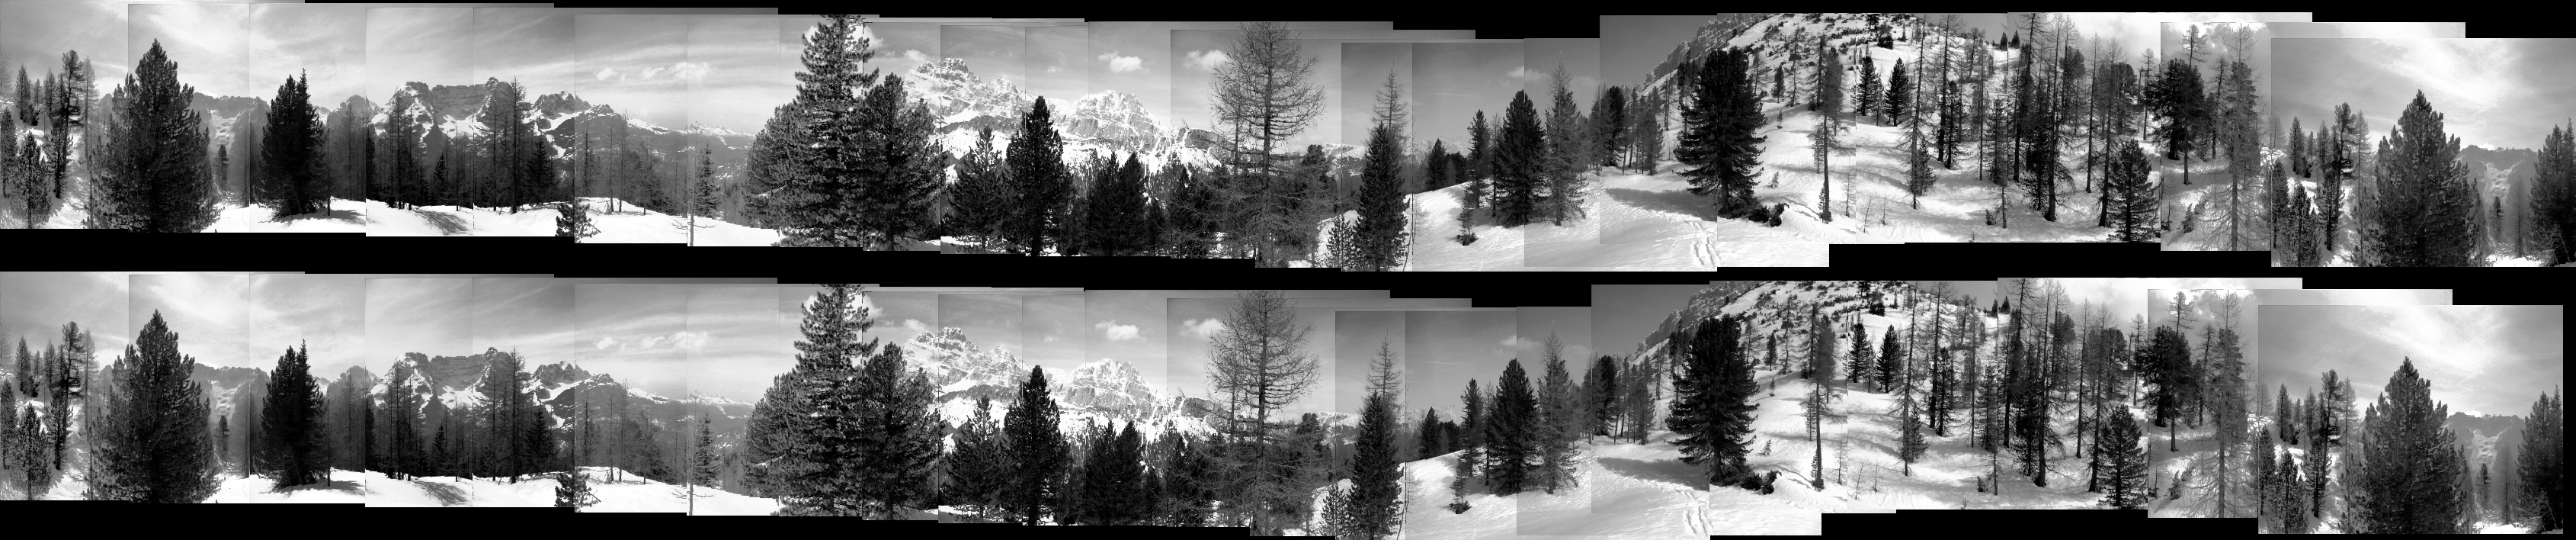
\includegraphics[width=170mm]{output1} 
\caption{\footnotesize{dataset\_dolomites/dolomites/}}
\end{center} 
\end{figure}
\begin{figure}[h]
\begin{center}
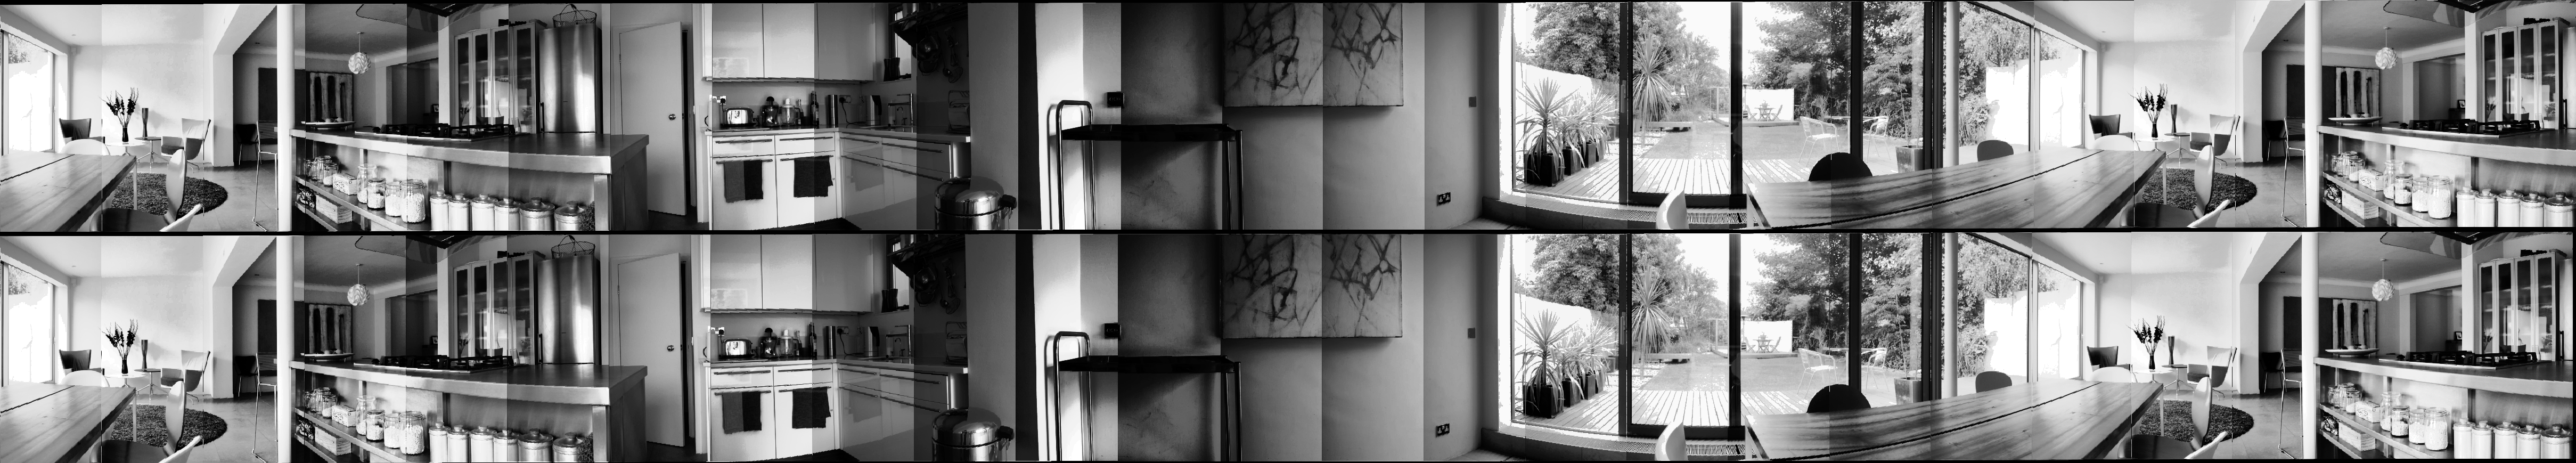
\includegraphics[width=170mm]{output2} 
\caption{\footnotesize{dataset\_kitchen/kitchen/.}}
\end{center} 
\end{figure}
\begin{figure}[h]
\begin{center}
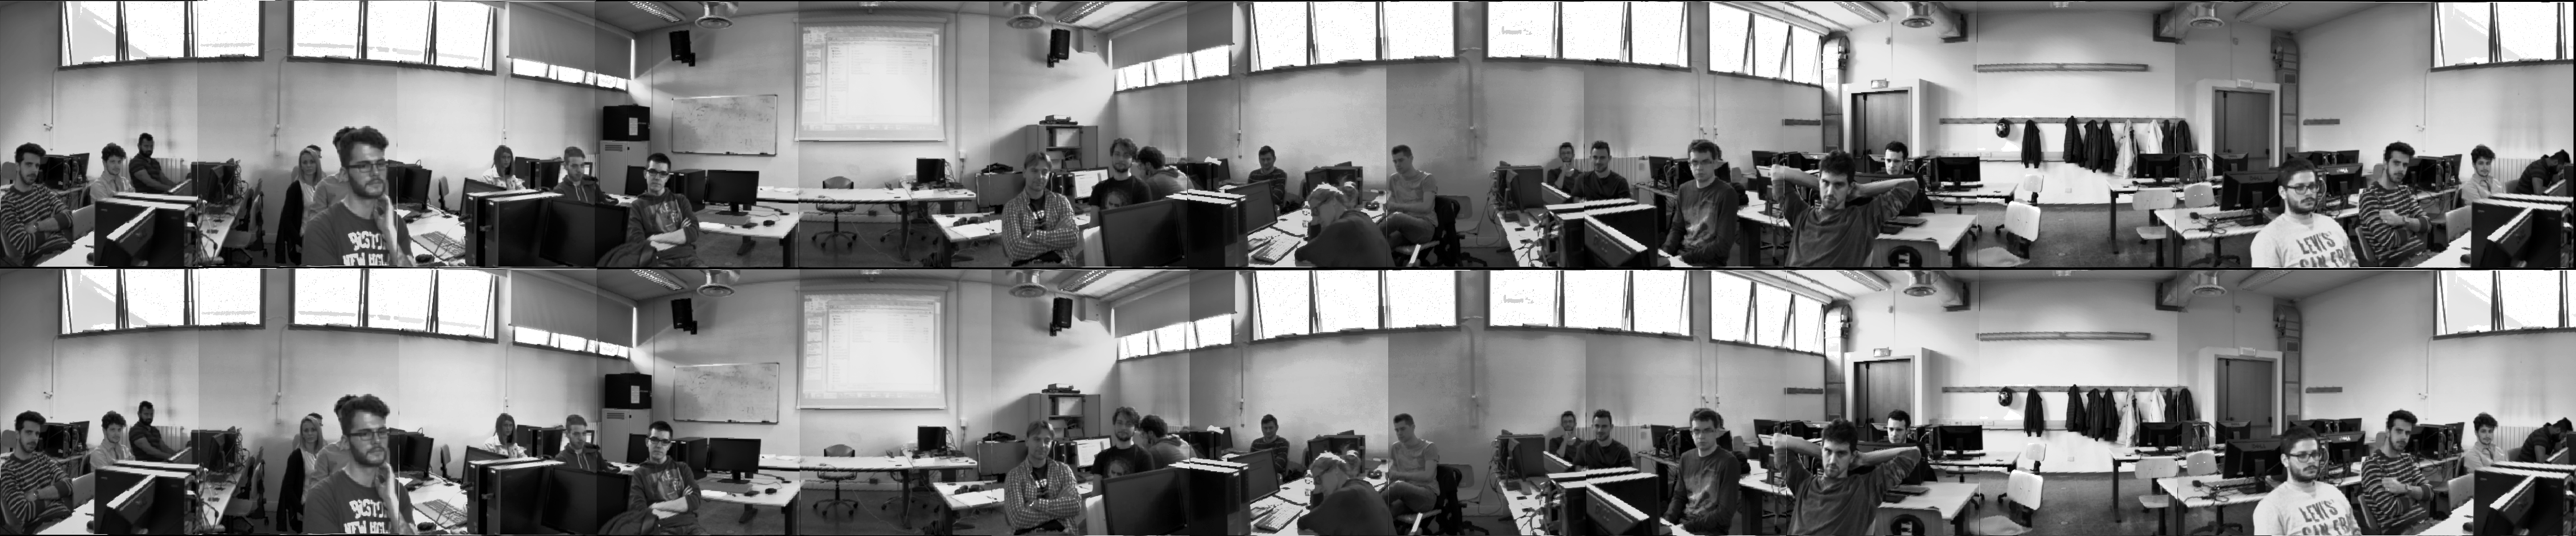
\includegraphics[width=170mm]{output3} 
\caption{\footnotesize{dataset\_lab/data/}}
\end{center} 
\end{figure}
\begin{figure}[H]
\begin{center}
\includegraphics[width=170mm]{output4} 
\caption{\footnotesize{dataset\_lab\_19\_automatic/.}}
\vspace{4mm}
\includegraphics[width=170mm]{output5} 
\caption{\footnotesize{dataset\_lab\_19\_manual/.}}
\end{center} 
\end{figure}

\end{document}